\begin{figure}[bht]
\centering
\tikzstyle{_BoldEdgeStyle} = [line width=3]
\begin{tikzpicture}[scale = 11]
\tikzstyle{VertexStyle} = []
\tikzstyle{EdgeStyle} = []
\tikzstyle{labeledStyle}=[shape = circle, minimum size = 6pt, inner sep = 1.2pt, draw]
\tikzstyle{unlabeledStyle}=[shape = circle, minimum size = 6pt, inner sep = 1.2pt, draw, fill]
\Vertex[style = labeledStyle, x = 0.650, y = 0.550, L = \small {$0$}]{v0}
\Vertex[style = labeledStyle, x = 0.850, y = 0.700, L = \small {$0$}]{v1}
\Vertex[style = labeledStyle, x = 1.050, y = 0.550, L = \small {$0$}]{v2}
\Vertex[style = labeledStyle, x = 0.850, y = 0.950, L = \small {$1$}]{v3}
\Edge[label = \tiny {}, labelstyle={auto=right, fill=none}](v1)(v0)
\Edge[label = \tiny {}, labelstyle={auto=right, fill=none}](v1)(v2)
\Edge[style = _BoldEdgeStyle, label = \tiny {}, labelstyle={auto=right, fill=none}](v1)(v3)
\Edge[style = _BoldEdgeStyle, label = \tiny {}, labelstyle={auto=right, fill=none}](v3)(v0)
\Edge[style = _BoldEdgeStyle, label = \tiny {}, labelstyle={auto=right, fill=none}](v3)(v2)
\Edge[label = \tiny {}, labelstyle={auto=right, fill=none}](v2)(v0)
\end{tikzpicture}
\begin{tikzpicture}[scale = 11]
\tikzstyle{VertexStyle} = []
\tikzstyle{EdgeStyle} = []
\tikzstyle{labeledStyle}=[shape = circle, minimum size = 6pt, inner sep = 1.2pt, draw]
\tikzstyle{unlabeledStyle}=[shape = circle, minimum size = 6pt, inner sep = 1.2pt, draw, fill]
\Vertex[style = labeledStyle, x = 0.650, y = 0.550, L = \small {$0$}]{v0}
\Vertex[style = labeledStyle, x = 0.850, y = 0.700, L = \small {$0$}]{v1}
\Vertex[style = labeledStyle, x = 1.050, y = 0.550, L = \small {$0$}]{v2}
\Vertex[style = labeledStyle, x = 0.850, y = 0.950, L = \small {$1$}]{v3}
\Vertex[style = labeledStyle, x = 0.750, y = 0.750, L = \small {$0$}]{v4}
\Vertex[style = labeledStyle, x = 0.850, y = 0.800, L = \small {$0$}]{v5}
\Vertex[style = labeledStyle, x = 0.950, y = 0.750, L = \small {$0$}]{v6}
\Edge[label = \tiny {}, labelstyle={auto=right, fill=none}](v1)(v0)
\Edge[label = \tiny {}, labelstyle={auto=right, fill=none}](v1)(v2)
\Edge[label = \tiny {}, labelstyle={auto=right, fill=none}](v2)(v0)
\Edge[style = _BoldEdgeStyle, label = \tiny {}, labelstyle={auto=right, fill=none}](v5)(v3)
\Edge[style = _BoldEdgeStyle, label = \tiny {}, labelstyle={auto=right, fill=none}](v5)(v1)
\Edge[style = _BoldEdgeStyle, label = \tiny {}, labelstyle={auto=right, fill=none}](v4)(v3)
\Edge[style = _BoldEdgeStyle, label = \tiny {}, labelstyle={auto=right, fill=none}](v4)(v0)
\Edge[style = _BoldEdgeStyle, label = \tiny {}, labelstyle={auto=right, fill=none}](v6)(v3)
\Edge[style = _BoldEdgeStyle, label = \tiny {}, labelstyle={auto=right, fill=none}](v6)(v2)
\end{tikzpicture}
\begin{tikzpicture}[scale = 11]
\tikzstyle{VertexStyle} = []
\tikzstyle{EdgeStyle} = []
\tikzstyle{labeledStyle}=[shape = circle, minimum size = 6pt, inner sep = 1.2pt, draw]
\tikzstyle{unlabeledStyle}=[shape = circle, minimum size = 6pt, inner sep = 1.2pt, draw, fill]
\Vertex[style = labeledStyle, x = 1.000, y = 0.250, L = \small {$0$}]{v0}
\Vertex[style = labeledStyle, x = 1.200, y = 0.250, L = \small {$0$}]{v1}
\Vertex[style = labeledStyle, x = 0.850, y = 0.400, L = \small {$0$}]{v2}
\Vertex[style = labeledStyle, x = 1.000, y = 0.400, L = \small {$0$}]{v3}
\Vertex[style = labeledStyle, x = 1.350, y = 0.400, L = \small {$0$}]{v4}
\Vertex[style = labeledStyle, x = 1.200, y = 0.400, L = \small {$0$}]{v5}
\Vertex[style = labeledStyle, x = 1.100, y = 0.600, L = \small {$1$}]{v6}
\Edge[label = \small {}, labelstyle={auto=right, fill=none}](v0)(v2)
\Edge[label = \small {}, labelstyle={auto=right, fill=none}](v0)(v3)
\Edge[label = \small {}, labelstyle={auto=right, fill=none}](v1)(v0)
\Edge[label = \small {}, labelstyle={auto=right, fill=none}](v2)(v3)
\Edge[label = \small {}, labelstyle={auto=right, fill=none}](v4)(v1)
\Edge[label = \small {}, labelstyle={auto=right, fill=none}](v5)(v1)
\Edge[label = \small {}, labelstyle={auto=right, fill=none}](v5)(v4)
\Edge[label = \small {}, labelstyle={auto=right, fill=none}](v6)(v2)
\Edge[label = \small {}, labelstyle={auto=right, fill=none}](v6)(v3)
\Edge[label = \small {}, labelstyle={auto=right, fill=none}](v6)(v4)
\Edge[label = \small {}, labelstyle={auto=right, fill=none}](v6)(v5)
\end{tikzpicture}


\caption{Three pairs $(G,h_x)$ that are in $\D$.  In each case $x$ is labeled 1
and all other vertices are labeled 0.  Each other pair in $\D$ can be formed
from one of these pairs by repeatedly stretching one or more bold edges.}
\label{fig:seeds}
\end{figure}

